\documentclass[11pt]{article}
\usepackage[margin=1in]{geometry}
\usepackage{graphicx}
\usepackage{amsmath}
\usepackage{booktabs}

\title{A Finite Intercept Correction Calculation}
\author{Anonymous}
\date{}

\begin{document}
\maketitle

\begin{abstract}
This worked teaching note connects residual arithmetic, error measurement, and evaluation dependencies. On five synthetic observations with targets $y=2x+3$, the fixed predictor $2x$ has residual $3$ at every input. Adding the observed mean residual gives exact agreement with those targets. Three recorded correction settings illustrate how absolute and squared errors respond to a shared offset. A measured error table, discrete MSE plot, and residual-flow diagram present the calculation together with the reuse of the observations for estimation and evaluation.
\end{abstract}

\section{Introduction}

This note is intended for students learning to distinguish a fixed prediction rule, an estimated adjustment, and the observations used to assess the result. Its contribution is instructional: one fully specified calculation connects these three objects through equations, a numerical table, and two complementary figures. The arithmetic is deliberately immediate so that readers can inspect the data dependencies alongside the reported errors.

The exercise starts with a supplied slope and a constant discrepancy. Readers first calculate residuals, then average them to obtain an additive correction, and finally compare the corrected predictions with the original targets. This sequence makes the meaning of exact agreement concrete: the reported error describes the same five observations that determine the correction. The intermediate correction also provides a direct comparison between absolute and squared error.

\section{Related Work}

Residual examination provides graphical and numerical ways to assess fitted analyses \cite{Anscombe1963ExaminationAnalysis}. Here, listing every residual makes the shared discrepancy visible without additional diagnostics. Regression through the origin supplies a related instructional setting \cite{Eisenhauer2003RegressionThrough}; in this exercise, however, the slope is specified in advance, and the calculated quantity is an additive offset.

The distinction between explanatory and predictive modeling discussed by Shmueli \cite{Shmueli2010ExplainOr} motivates attention to what an error calculation assesses. The present example describes agreement on explicitly listed observations. Its teaching objective is to connect that agreement to the observations used in constructing the adjustment.

\section{Method}

\subsection{Finite Inputs and Fixed Predictor}

The five constructed observations and baseline predictions, in their supplied order, are
\[
\begin{aligned}
x&=(-2,-1,0,1,2),\\
y&=(-1,1,3,5,7),\\
\widehat{y}^{(0)}&=(-4,-2,0,2,4).
\end{aligned}
\]
The baseline rule is $\widehat{y}^{(0)}_i=2x_i$, while the targets satisfy
$y_i=2x_i+3$. Subtracting predictions from targets gives
\[
r_i=y_i-2x_i=3,\qquad i=1,\ldots,5.
\]
Thus, each baseline prediction falls below its target by the same amount.

\subsection{Mean-Residual Correction and Data Dependencies}

The observed mean residual supplies the correction:
\[
b=\frac{1}{5}\sum_{i=1}^{5}r_i
 =\frac{3+3+3+3+3}{5}=3.
\]
Keeping the supplied slope fixed gives
\[
\widehat{y}^{(b)}_i=2x_i+b=2x_i+3=y_i.
\]
Exact agreement follows from substituting the common residual into the corrected prediction.

Figure~\ref{fig:residual_workflow} traces this calculation. Targets and baseline predictions jointly determine the residuals; their mean determines $b$; and the corrected predictions are compared with the original targets. The dashed connection identifies observation reuse. The arithmetic was implemented in base R \cite{Ihaka1996RLanguage}, and every numerical input needed to reproduce it is stated above.

\begin{figure}[tbp]
\centering
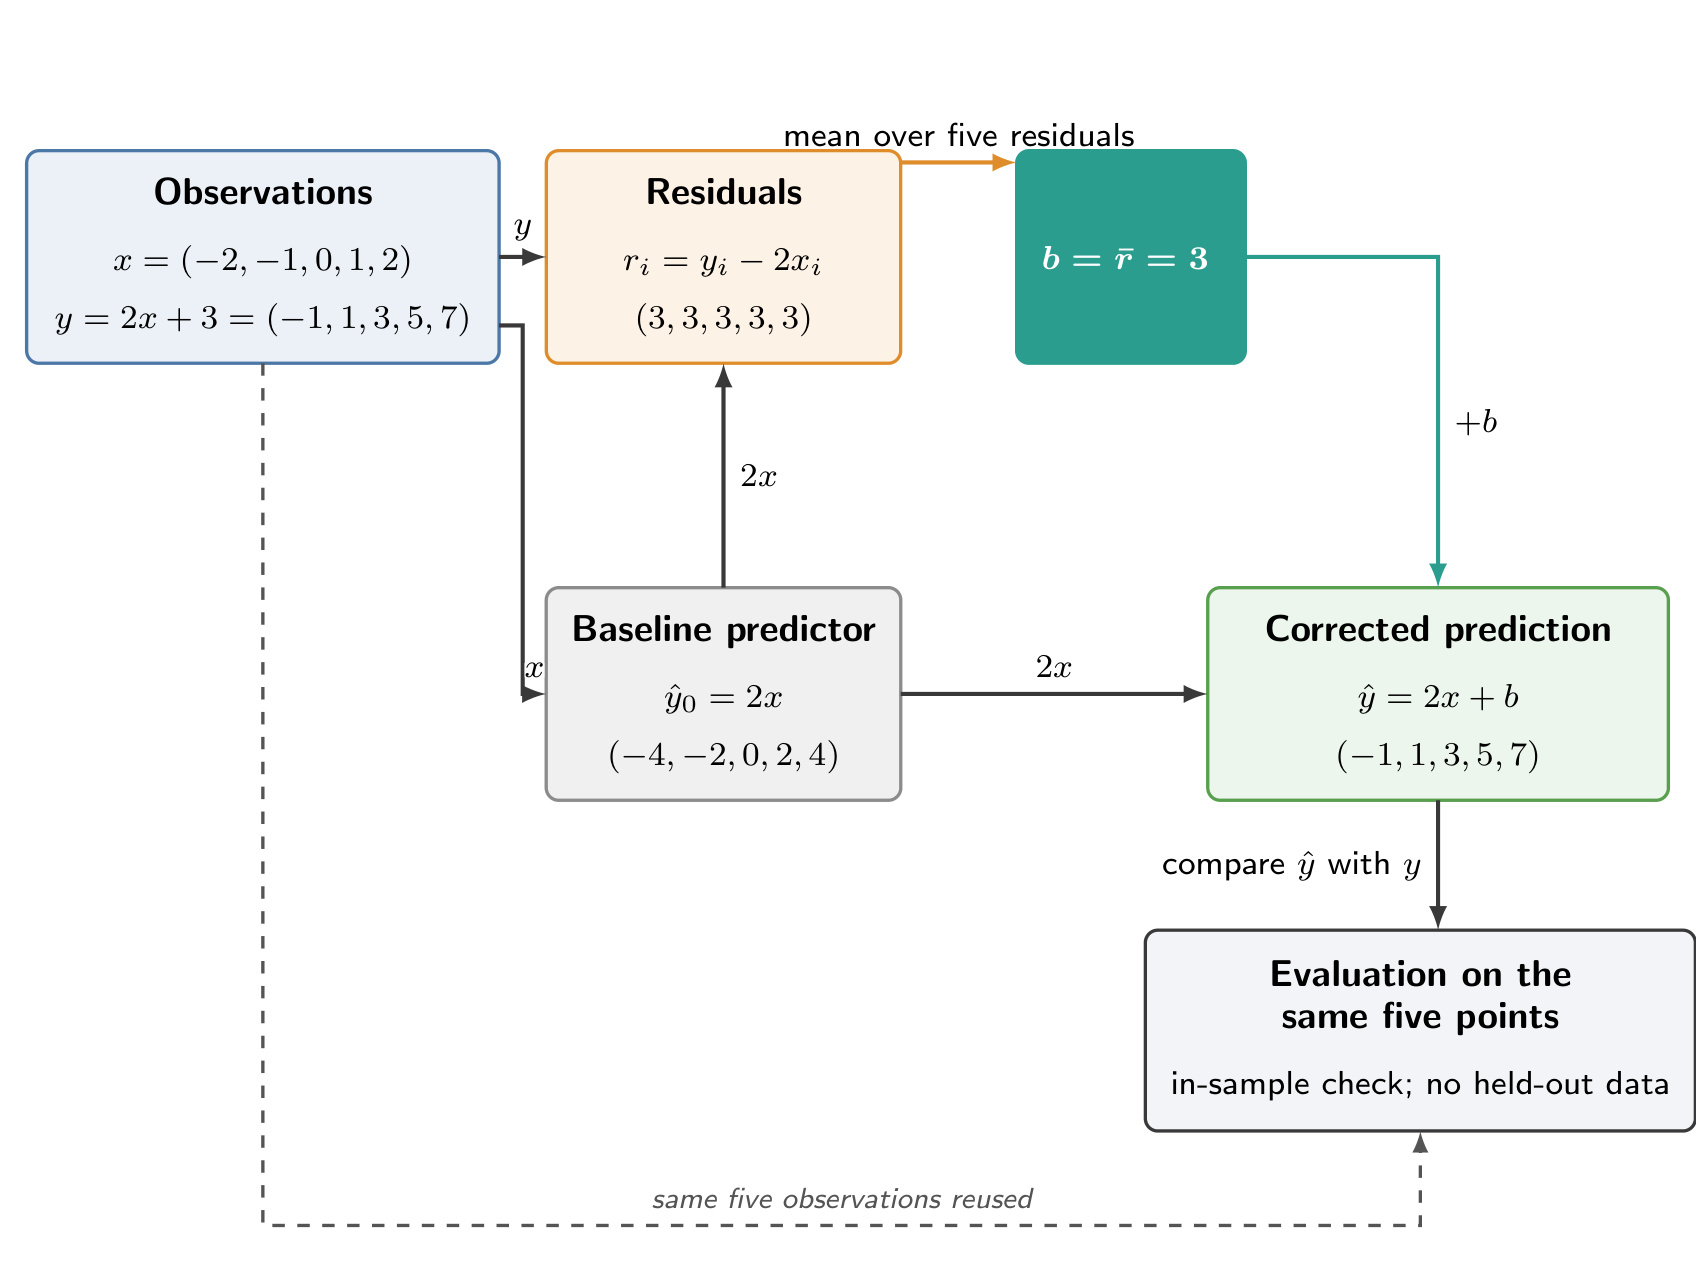
\includegraphics[width=\linewidth]{figures/fig_residual_workflow.jpg}
\caption{Residual-flow diagram for the supplied calculation. Five residuals equal to $3$ determine $b=3$. The dashed connection shows that the original observations also supply the evaluation targets.}
\label{fig:residual_workflow}
\end{figure}

\section{Experiments}

\subsection{Recorded Calculation and Error Definitions}

The experimental record contains one deterministic calculation at the three supplied settings $b=0$, $1.5$, and $3$. For each setting, define
\[
e_i(b)=y_i-(2x_i+b),
\]
\[
\operatorname{MAE}(b)=\frac{1}{5}\sum_{i=1}^{5}|e_i(b)|,
\qquad
\operatorname{MSE}(b)=\frac{1}{5}\sum_{i=1}^{5}e_i(b)^2.
\]
For these observations, substitution gives
\[
e_i(b)=3-b,\qquad
\operatorname{MAE}(b)=|3-b|,\qquad
\operatorname{MSE}(b)=(3-b)^2.
\]
These identities explain the recorded values algebraically. The settings are comparison values for the added scalar, rather than successive optimization steps.

\subsection{Measured Errors and Visualization}

Table~\ref{tab:recorded_errors} reports all three recorded settings. At $b=0$, every difference is $3$, giving MAE $3$ and MSE $9$. At $b=3$, each difference is zero.

The instructional role of $b=1.5$ is to separate the behavior of the two error measures. It removes half the original discrepancy at every observation: the remaining absolute difference is $1.5$, while its square is $2.25$. Readers can therefore check how the same partial correction appears under absolute and squared loss. This setting is a supplied comparison; the observed mean-residual correction remains $b=3$.

\begin{table}[tbp]
\centering
\caption{Complete recorded errors. All entries are calculated on the five observations used to determine the mean-residual correction.}
\label{tab:recorded_errors}
\begin{tabular}{rrr}
\toprule
Added $b$ & Mean absolute error & Mean squared error \\
\midrule
0   & 3   & 9    \\
1.5 & 1.5 & 2.25 \\
3   & 0   & 0    \\
\bottomrule
\end{tabular}
\end{table}

Figure~\ref{fig:intercept_error} displays exactly the three recorded MSE pairs. Its discrete points keep the measured settings visible, while the algebra above explains their values. Read together, the plot and flow diagram connect error magnitude to the calculation that produces the correction and to the observations on which the errors are assessed.

\begin{figure}[tbp]
\centering
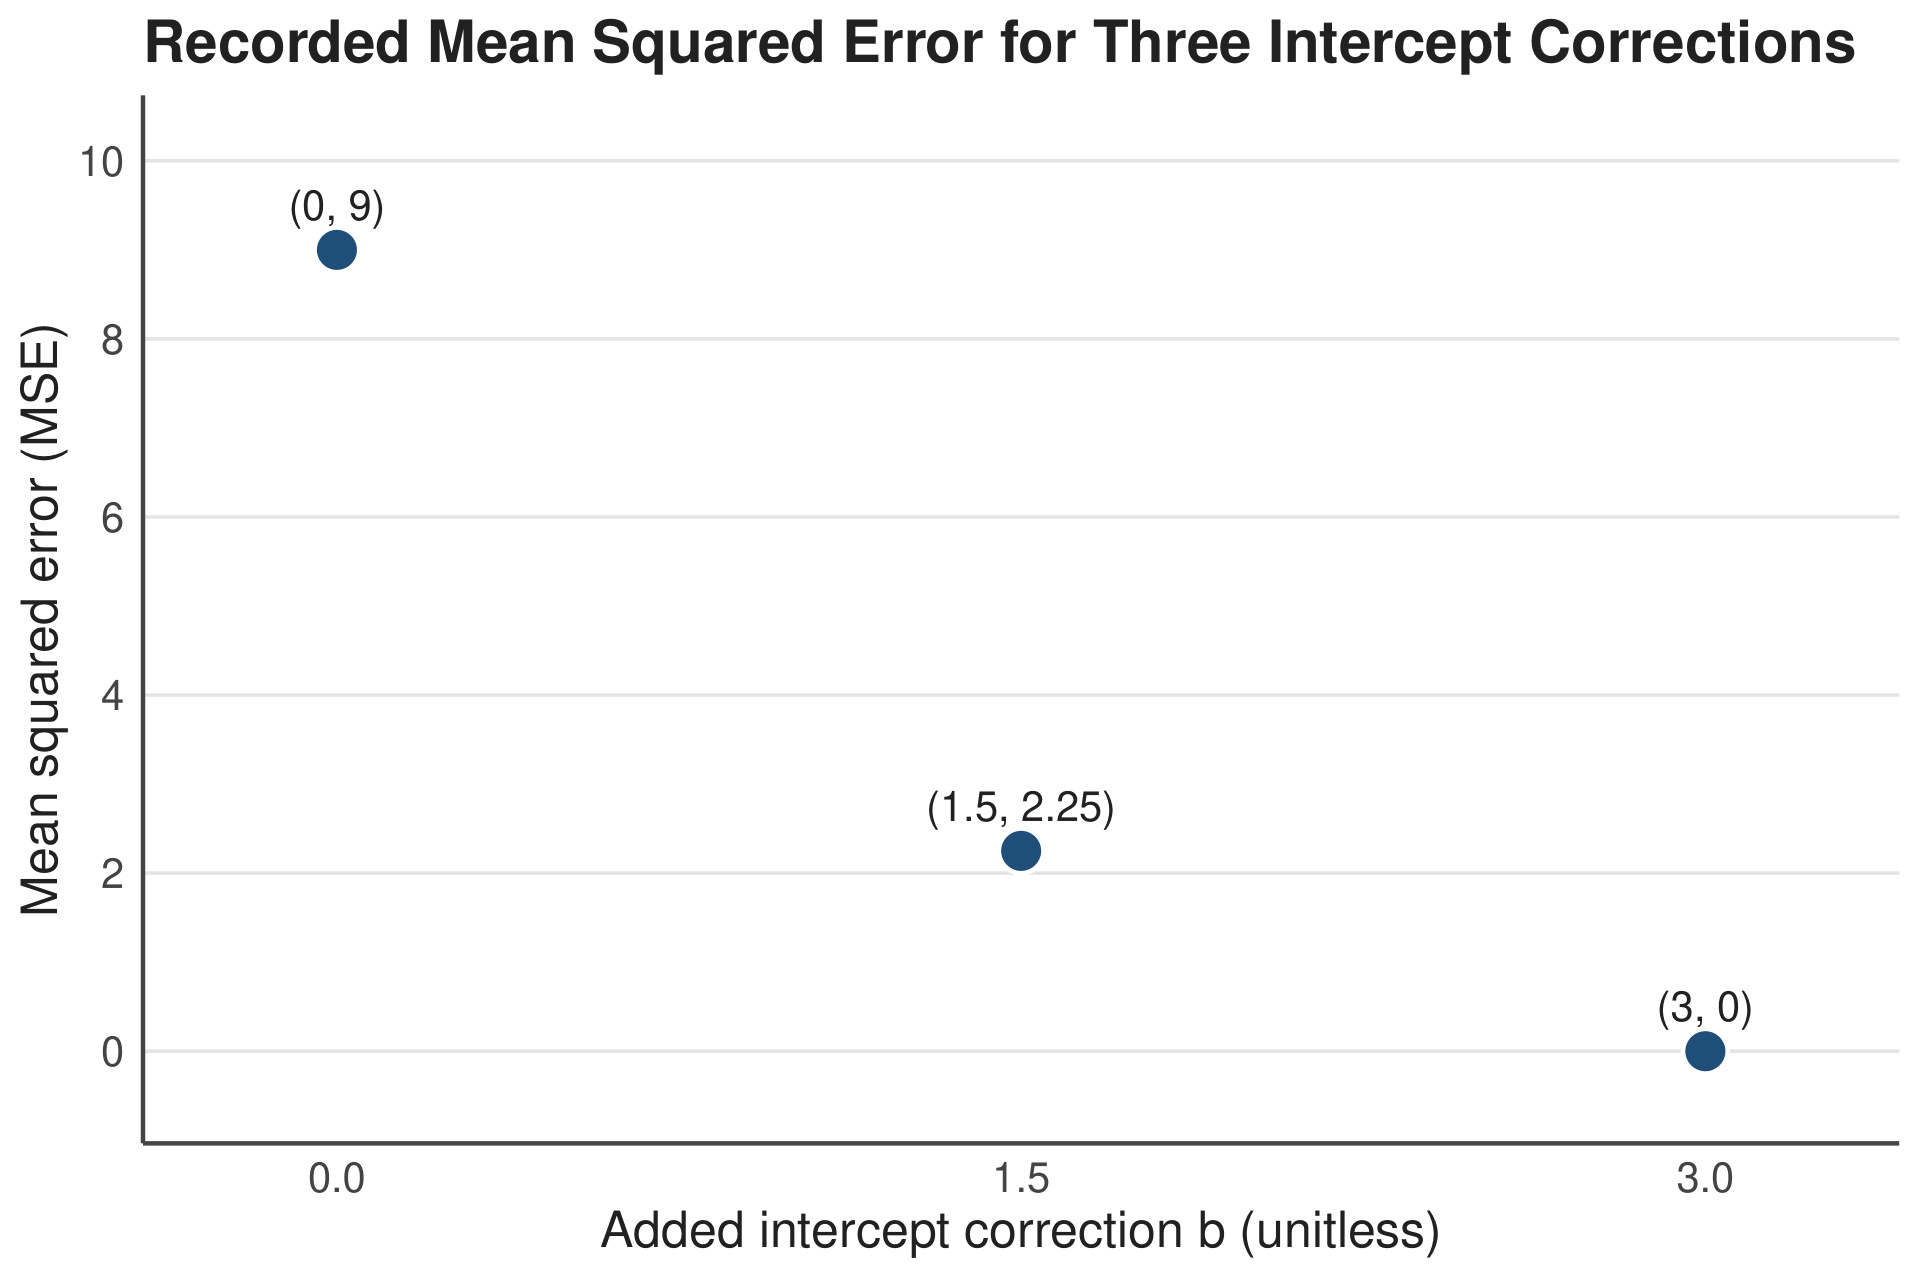
\includegraphics[width=\linewidth]{figures/fig_intercept_error.jpg}
\caption{Recorded MSE at $(b,\operatorname{MSE})=(0,9)$, $(1.5,2.25)$, and $(3,0)$. Labels identify the measured pairs; each error evaluates the same five observations.}
\label{fig:intercept_error}
\end{figure}

\section{Conclusion}

The example links a common residual, its mean, and the resulting prediction errors in a calculation that can be checked observation by observation. The partial correction distinguishes absolute from squared loss, and the flow diagram identifies the shared observations behind estimation and evaluation. Together, these elements provide a compact exercise in interpreting an exact fit through its arithmetic and data dependencies.


\begin{thebibliography}{9}

\bibitem{Anscombe1963ExaminationAnalysis}
Francis John Anscombe and John W. Tukey.
\newblock The Examination and Analysis of Residuals.
\newblock \emph{Technometrics}, 1963.

\bibitem{Eisenhauer2003RegressionThrough}
Joseph G. Eisenhauer.
\newblock Regression through the Origin.
\newblock \emph{Teaching Statistics}, 2003.

\bibitem{Shmueli2010ExplainOr}
Galit Shmueli.
\newblock To Explain or to Predict?
\newblock \emph{Statistical Science}, 2010.

\bibitem{Ihaka1996RLanguage}
Ross Ihaka and Robert C. Gentleman.
\newblock R: A Language for Data Analysis and Graphics.
\newblock \emph{Journal of Computational and Graphical Statistics}, 1996.

\end{thebibliography}

% PAPER_ORCHESTRA_PROVENANCE_BEGIN
\clearpage
\section*{Figure source provenance}
The files below are the exact sources that produced the embedded figure previews. Paths are relative to this manuscript's source directory. The accompanying \texttt{figure\char95{}provenance.json} records all artifact checksums.\par
\medskip\noindent\textbf{Figure~\ref{fig:intercept_error} (\texttt{fig\char95{}intercept\char95{}error.jpg}).}\par
\noindent R/ggplot2 source: \texttt{figure\char95{}code/\allowbreak{}fig\char95{}intercept\char95{}error/\allowbreak{}source.R}.\par
\noindent Source SHA256: \texttt{34ba57e5\allowbreak{}6adf6b78\allowbreak{}4bfabe24\allowbreak{}299ef6d2\allowbreak{}5ce74051\allowbreak{}70d96d8c\allowbreak{}09ada698\allowbreak{}97622aee}.\par
\noindent Rendering metadata: \texttt{figure\char95{}code/\allowbreak{}fig\char95{}intercept\char95{}error/\allowbreak{}render.json}.\par
\noindent Exact export wrapper: \texttt{figure\char95{}code/\allowbreak{}fig\char95{}intercept\char95{}error/\allowbreak{}worker.R}.\par
\noindent Wrapper SHA256: \texttt{1aedad4b\allowbreak{}1547d4b2\allowbreak{}d394cbb0\allowbreak{}239655d3\allowbreak{}667d453d\allowbreak{}d1fd0eca\allowbreak{}3e77c037\allowbreak{}e6d34892}.\par
\noindent Rendering metadata: \texttt{figure\char95{}code/\allowbreak{}fig\char95{}intercept\char95{}error/\allowbreak{}sessionInfo.txt}.\par
\medskip\noindent\textbf{Figure~\ref{fig:residual_workflow} (\texttt{fig\char95{}residual\char95{}workflow.jpg}).}\par
\noindent LaTeX/TikZ source: \texttt{figure\char95{}code/\allowbreak{}fig\char95{}residual\char95{}workflow/\allowbreak{}source.tex}.\par
\noindent Source SHA256: \texttt{e1de201d\allowbreak{}70c4a996\allowbreak{}77d8214a\allowbreak{}b33a2f9c\allowbreak{}6815b281\allowbreak{}a8c5bf20\allowbreak{}97e46cce\allowbreak{}5855da92}.\par
\noindent Rendering metadata: \texttt{figure\char95{}code/\allowbreak{}fig\char95{}residual\char95{}workflow/\allowbreak{}render.json}.\par
% PAPER_ORCHESTRA_PROVENANCE_END
\end{document}